% \documentclass{article}
% \usepackage[utf8]{inputenc}

\documentclass{assignment format}
\usepackage{assignment}
\usepackage{bm}
\setcounter{section}{-1}
\setcounter{subsection}{-1}
\usepackage[cjk]{kotex}
\usepackage{amsmath, amsthm, amssymb}
\usepackage{enumerate}
\usepackage{enumitem}
\usepackage{amsfonts}
\usepackage[dvipsnames]{xcolor}
\usepackage{url}
\usepackage{graphicx}
\usepackage{float} 
\usepackage{physics}
\usepackage{bbm}
\usepackage{caption}
\usepackage{minted}
\usepackage{todonotes}
\usepackage{relsize}
\usepackage{float}
\usepackage{blindtext}
\usepackage{multicol}
\newcommand{\note}[4][]{\todo[author=#2,color=#3,size=\scriptsize,fancyline,caption={},#1]{#4}} % default note settings, used by macros below.
\newcommand{\mrinmaya}[2][]{\note[#1]{mrinmaya}{blue!40}{#2}}

\usepackage[colorlinks=true]{hyperref}

\DeclareMathOperator*{\argmax}{arg\,max}
\newcommand{\alns}[1] {
	\begin{align*} #1 \end{align*}
}

\newcommand{\pd}[2] {
 \frac{\partial #1}{\partial #2}
}
\renewcommand{\Re} { \mathbb{R} }
\newcommand{\btx} { \mathbf{\tilde{x}} }
\newcommand{\bth} { \mathbf{\tilde{h}} }
\newcommand{\smx} { \operatorname{softmax} }
\newcommand{\relu} { \operatorname{ReLU} }
\newcommand{\sigmoid} { \operatorname{\sigma} }
\newcommand{\CE} { \operatorname{CE} }
\newcommand{\byt} { \hat{\by} }
\newcommand{\yt} { \hat{y} }

\newcommand{\oft}[1]{^{(#1)}}
\newcommand{\fone}{\ensuremath{F_1}}

\newcommand{\ac}[1]{ {\color{red} \textbf{AC:} #1} }
\newcommand{\ner}[1]{\textbf{\color{blue} #1}}

\definecolor{mygreen}{rgb}{0,0.6,0}
\newcommand{\ml}[1]{\textcolor{mygreen}{\textbf{Mina:} #1}}
% real numbers R symbol
\newcommand{\Real}{\mathbb{R}}

% encoder hidden
\newcommand{\henc}{\mathbf{h}^{\text{enc}}}
\newcommand{\hencfw}[1]{\overrightarrow{\mathbf{h}^{enc}_{#1}}}
\newcommand{\hencbw}[1]{\overleftarrow{\mathbf{h}^{enc}_{#1}}}

% encoder cell
\newcommand{\cenc}{\mathbf{c}^{\text{enc}}}
\newcommand{\cencfw}[1]{\overrightarrow{\mathbf{c}^{enc}_{#1}}}
\newcommand{\cencbw}[1]{\overleftarrow{\mathbf{c}^{enc}_{#1}}}

% decoder hidden
\newcommand{\hdec}{\mathbf{h}^{\text{dec}}}

% decoder cell
\newcommand{\cdec}{\mathbf{c}^{\text{dec}}}
\newenvironment{answer}{
    {\bf Answer:} \begingroup\color{red}
}{\endgroup}%
\begin{document}


\makeheader{\textbf{Due on} Thursday Oct. 24, 2024 \\ by \textbf{23:59 pm}}{Assignment 3: Recurrent Neural Networks}
\begin{center}
%%%%%YOUR NAME HERE%%%%%

\fbox{%
  \parbox{\textwidth}{
  \begin{center}
\large\textbf{Honor Pledge for Graded Assignments}
\\
\\ 
   \large{ “I, YOUR NAME HERE , affirm that I have not given or received any unauthorized help on this assignment, and that this work is my own.”}
    \end{center}
}%
}
\end{center}

\section{Instructions}
\begin{itemize}
\item Total score cannot exceed 100 points. For example, if you score 98 points from non-bonus questions and 3 points are added from bonus questions, your score will be 100 points, not 101 points.
\item Skeleton codes for problem 3 are at the directory \texttt{/q3}. 
\item Run the \texttt{bash collect\_submission.sh} script to produce your 2000\_00000\_coding.zip file. Please make sure to modify collect\_submission.sh file before running this command. (\textbf{2000\_00000} stands for your student id.)
\item Modify this tex file into \texttt{2000\_00000\_written.pdf} with your written solutions.
\item Upload both \texttt{2000\_00000\_coding.zip} and \texttt{2000\_00000\_written.pdf} to etl website.
\item \textbf{If the submission instructions are not followed, \texttt{4 points} will be deducted.}
\end{itemize}

\section{NLP tasks with RNN (20 pts)}
RNNs are versatile! In class, we learned that this family of neural networks have many important advantages and can be used in a variety of tasks. They are commonly used in many state-of-the-art architectures for NLP.

For each of the following tasks, state how you would run RNN to do that task. In particular, specify how the RNN would be used at test time (not training time), and specify
\begin{itemize}
    \item How many outputs i.e. number of times the softmax $\hat{y}^{(t)}$ is called from your RNN. If the number of outputs is not fixed, state it as arbitrary.  
    \item What each $\hat{y}^{(t)}$ is a probability distribution over (e.g. distributed over all species of categories).
    \item Which inputs are fed to produce each output $\hat{y}^{(t)}$.
    \end{itemize}
The inputs for each of the tasks are specified below.
\begin{enumerate}[label=(\alph*)]
    \item \textbf{Movie Rating (5 pts)}: Classify sentiment of a movie review ranging from negative to positive (integer values from 1 to 5).\\Inputs: A sentence containing n words.
    \begin{answer}
    \end{answer}
    \item \textbf{Part-of-speech Tagging (5 pts)}: For each word in a sentence, categorize that word in correspondence with a particular part-of-speech such as either nouns, verbs, adjectives, adverbs, etc.\\Inputs: A sentence containing n words.
    \begin{answer}
    \end{answer}
    \item \textbf{Text Generation (5 pts)}: Generate text from a chatbot that was trained to speak like a news anchor by predicting the next word in the sequence. \\Input: A single start word or token that is fed into the first time step of the RNN.
    \begin{answer}
    \end{answer}
    \item \textbf{Machine Translation (5 pts)}: Translate the given sentence into another language. \\Input: A sentence containing n words. 
    \begin{answer}
    \end{answer}
    \end{enumerate}
    
\section{Backprop on LSTM (12 pts)}
In class, we learned about Long Short-Term Memory (LSTM) model. Recall the units of an LSTM cell are defined as
\begin{align*}
i_{t}=\sigma(W^{(i)}x_{t} + U^{(i)}h_{t-1})\\
f_{t}=\sigma(W^{(f)}x_{t} + U^{(f)}h_{t-1})\\
o_{t}=\sigma(W^{(o)}x_{t} + U^{(o)}h_{t-1})\\
\tilde{c_{t}} = tanh(W^{(c)}x_{t} + U^{(c)}h_{t-1})\\
c_{t} = f_{t}\circ c_{t-1}+i_{t}\circ \tilde{c_{t}}\\
h_{t}=o_{t}\circ tanh(c_{t})
\end{align*}
where the final output of the last lstm cell is defined by $\hat{y_{t}}=softmax(h_{t}W+b)$. The final cost function $J$ uses the cross-entropy loss. Consider an LSTM for two time steps, $t$ and $t-1$.
    \begin{center}
        \captionsetup{width=0.4\textwidth}
        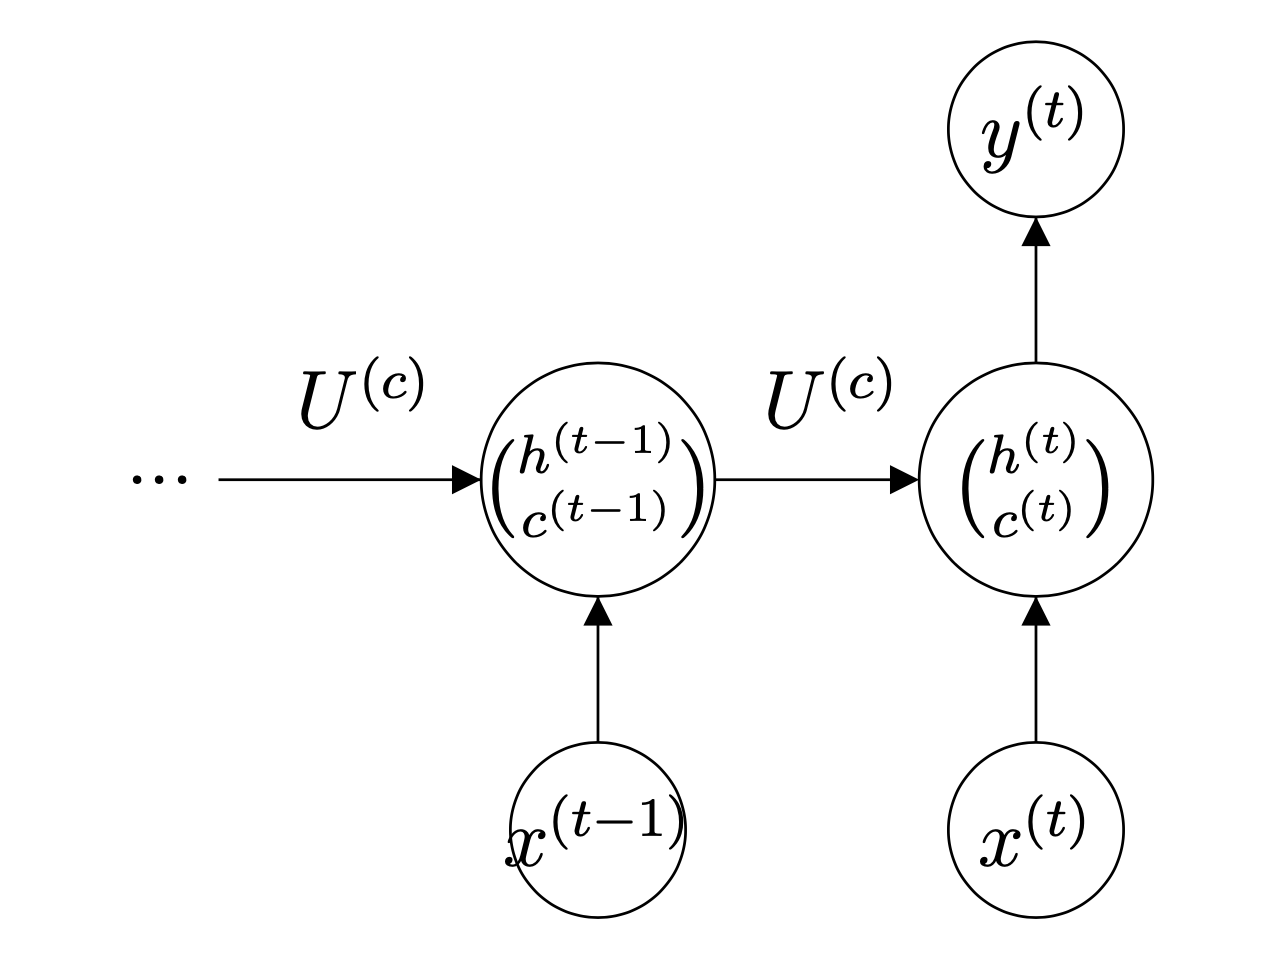
\includegraphics[width=0.4\textwidth]{LSTM.png}
        \label{LSTM-figure}
    \end{center}
\begin{enumerate}[label=(\alph*)]
    \item Derive the gradient $\frac{\delta J}{\delta U^{(c)}}$ in terms of the following gradients: $\frac{\delta h_{t}}{\delta h_{t-1}}, \frac{\delta h_{t-1}}{\delta U^{(c)}}, \frac{\delta J}{\delta h_{t}}, \frac{\delta c_{t}}{\delta U^{(c)}}, \frac{\delta c_{t-1}}{\delta U^{(c)}}, \frac{\delta c_{t}}{\delta c_{t-1}}, \frac{\delta h_{t}}{\delta c_{t}},$ and $\frac{\delta h_{t}}{\delta o_{t}}$. \textit{Not all of the gradients may be used.} You can leave the answer in the form of chain rule and do not have to calculate any individual gradients in your final result. \textbf{(8 pts)}
    \begin{answer}
    \end{answer}
    \item Which part of the gradient $\frac{\delta J}{\delta U^{(c)}}$ allows LSTM to mitigate the effect of the vanishing gradient problem? \textbf{(4 pts)}
    \begin{answer}
    \end{answer}
\end{enumerate}

\section{Neural Machine Translation with LSTM (68$+$3 pts)}
 In Neural Machine Translation (NMT), our goal is to convert a sentence from the \textit{source} language to the \textit{target} language. In this assignment, we will implement a sequence-to-sequence (Seq2Seq) network with attention, to build a Neural Machine Translation (NMT) system between Jeju dialect and Korean. 
 \subsection{Training Procedure}
\begin{figure}[h]
    \begin{center}
        \captionsetup{width=0.8\textwidth}
        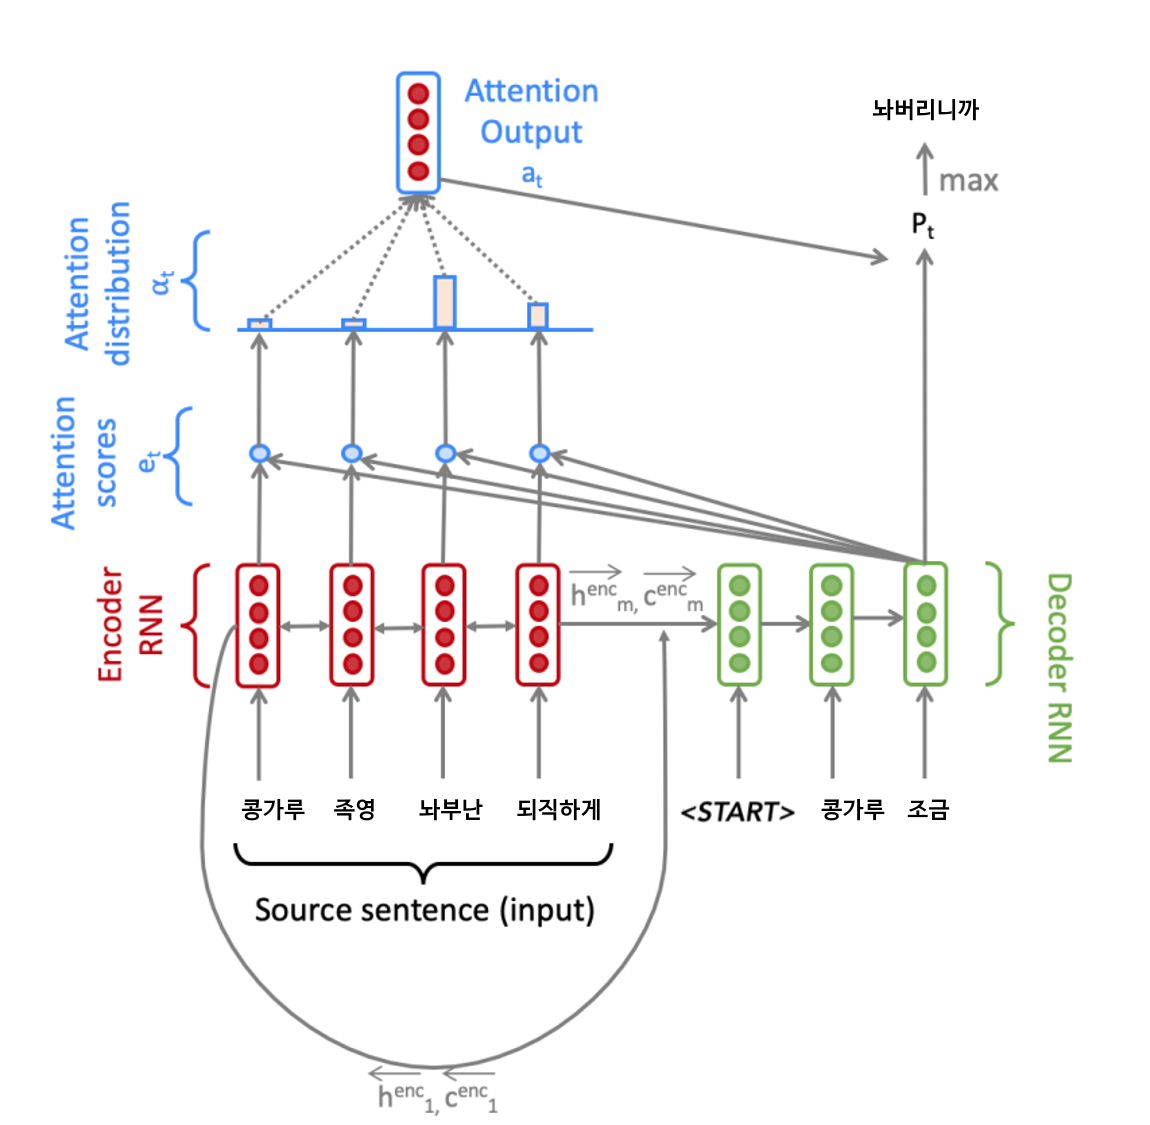
\includegraphics[width=0.7\textwidth]{nmt.png}
        \caption{Seq2Seq Model with Multiplicative Attention, shown on the third step of the decoder.  (NOTE: Embedding of NMT in the assignment differs from described above.)
        }
        \label{nmt-figure}
    \end{center}
\end{figure}
In this section, we describe the \textbf{training procedure} for the proposed NMT system, which uses a Bidirectional LSTM Encoder and a Unidirectional LSTM Decoder. The model is trained and evaluated on JIT (Jejueo interview transcripts) dataset\footnote{\url{https://www.kaggle.com/datasets/bryanpark/jit-dataset}}. Given a sentence in the source language (Jeju dialect), we look up the subword embeddings from an embeddings matrix, yielding $\mathbf{x}_1, \dots, \mathbf{x}_m$ ($\mathbf{x}_i \in \mathbb{R}^{e \times 1}$), where $m$ is the length of the source sentence and $e$ is the embedding size. We feed these embeddings to the bidirectional encoder, yielding hidden states and cell states for both the forwards ($\rightarrow$) and backwards ($\leftarrow$) LSTMs. The forwards and backwards versions are concatenated to make hidden states $\mathbf{h}^{enc}_i$ and cell states $\mathbf{c}^{enc}_i$:

\begin{align}
    \henc_i = [\hencbw{i}; \hencfw{i}] \enspace &\text{where}\enspace \henc_i \in \Real^{2h \times 1}, \hencbw{i}, \hencfw{i} \in \Real^{h \times 1} &1 \le i \le m \\
    \cenc_i = [\cencbw{i}; \cencfw{i}] \enspace &\text{where} \enspace \cenc_i \in \Real^{2h \times 1}, \cencbw{i}, \cencfw{i} \in \Real^{h \times 1} &1 \le i \le m
\end{align}
We then initialize the decoder's first hidden state $\hdec_0$ and cell state $\cdec_0$ with a linear projection of the encoder's final hidden state and final cell state.\footnote{Note that we regard $[\hencbw{1}, \hencfw{m}]$ as the `final hidden state' of the Encoder.} 

\begin{align}
    \hdec_0 = \mathbf{W}_{h}[\hencbw{1}; \hencfw{m}] \enspace &\text{where} \enspace \hdec_0 \in \Real^{h \times 1}, \mathbf{W}_{h} \in \Real^{h \times 2h}\\
    \cdec_0 = \mathbf{W}_{c}[\cencbw{1}; \cencfw{m}] \enspace &\text{where} \enspace \cdec_0 \in \Real^{h \times 1}, \mathbf{W}_{c} \in \Real^{h \times 2h}
\end{align}


With the decoder initialized, we must now feed it a target sentence. On the $t^{th}$ step, we look up the embedding for the $t^{th}$ subword,  $\mathbf{y}_t \in \Real^{e \times 1}$. We then concatenate $\mathbf{y}_t$ with the \textit{combined-output vector} $\mathbf{o}_{t-1} \in \Real^{h \times 1}$ from the previous timestep (we will explain what this is later down this page!\@) to produce $\overline{\mathbf{y}_t} \in \Real^{(e+h) \times 1}$. Note that for the first target subword (i.e. the start token) $\mathbf{o}_{0}$ is a zero-vector. We then feed $\overline{\mathbf{y}_t}$ as input to the decoder. 

\begin{align}
    \hdec_t, \cdec_t = \text{Decoder}(\overline{\mathbf{y}_t}, \hdec_{t-1}, \cdec_{t-1}) \enspace &\text{where} \enspace \hdec_t \in \Real^{h \times 1}, \cdec_t \in \Real^{h \times 1}\\
\end{align}
We then use $\hdec_t$ to compute  multiplicative attention over $\henc_1, \dots, \henc_m$:

\begin{align}
    \mathbf{e}_{t, i} = (\hdec_t)^T\mathbf{W}_{\text{attProj}}\henc_i \enspace &\text{where} \enspace \mathbf{e}_{t} \in \Real^{m \times 1}, \mathbf{W}_{\text{attProj}}\in \Real^{h \times 2h} & 1 \le i \le m \\
    \alpha_t= \text{softmax}(\mathbf{e}_t) \enspace &\text{where} \enspace \alpha_t \in \Real^{m \times 1}\\
    \mathbf{a}_t = \sum_{i=1}^{m}\alpha_{t,i}\henc_i \enspace &\text{where} \enspace \mathbf{a}_t \in \Real^{2h \times 1}
\end{align}
 
Here, $\mathbf{e}_{t, i}$ is a scalar, the $i^{th}$ element of $\mathbf{e}_{t} \in \Real^{m \times 1}$, computed using the hidden state of the decoder at the $t^{th}$ step $\hdec_t \in \Real^{h \times 1}$, the attention projection $\mathbf{W}_{\text{attProj}} \in \Real^{h \times 2h}$, and the hidden state of the encoder at the $i^{th}$ step $\henc_i \in \Real^{2h \times 1}$.

We now concatenate the attention output $\mathbf{a}_t$ with the decoder hidden state $\hdec_t$ and pass this through a linear layer, tanh, and dropout to attain the \textit{combined-output} vector $\mathbf{o}_{t}$.

\begin{align}   
    \mathbf{u}_{t} = [\mathbf{a}_{t}; \hdec_t] \enspace &\text{where} \enspace \mathbf{u}_t \in  \Real^{3h \times 1} \\
    \mathbf{v}_t = \mathbf{W}_{u}\mathbf{u}_t \enspace &\text{where} \enspace \mathbf{v}_t \in \Real^{h \times 1}, \mathbf{W}_{u} \in \Real^{h \times 3h}\\
    \mathbf{o}_t = \text{dropout}(\text{tanh}(\mathbf{v}_t)) \enspace &\text{where} \enspace \mathbf{o}_t \in \Real^{h \times 1}
\end{align}

Then, we produce a probability distribution $\mathbf{P}_t$ over target subwords at the $t^{th}$ timestep:

\begin{align}
    \mathbf{P}_t = \text{softmax}(\mathbf{W}_{\text{vocab}}\mathbf{o}_{t}) \enspace &\text{where} \enspace \mathbf{P}_t \in \Real^{V_{t} \times 1}, \mathbf{W}_{\text{vocab}} \in \Real^{V_{t} \times h}
\end{align}

Here, $V_{t}$ is the size of the target vocabulary. Finally, to train the network we compute the cross entropy loss between $\mathbf{P}_t$ and $\mathbf{g}_{t}$, where $\mathbf{g}_{t}$ is the one-hot vector of the target subword at the timestep $t$:

\begin{align}
    J_t(\theta) = \mathrm{CrossEntropy}(\mathbf{P}_t,\mathbf{g}_{t})
\end{align}

Here, $\theta$ represents all the parameters of the model and $J_t(\theta)$ is the loss on the step $t$ of the decoder.
Now that we have described the model, let's try implementing it for Jeju dialect to Korean translation!

\subsection{Setting up Virtual Environment}

In this part, we will set up a virtual environment for implementing the NMT machine. Please note that the following instructions are based on the gsds server as announced on the ETL board \footnote{\url{https://myetl.snu.ac.kr/courses/264449/discussion_topics/202254}}. Run the following commands within the assignment directory (\texttt{/q3}) to create the appropriate conda environment. This guarantees that you have all the necessary packages to complete the assignment. 

\begin{minted}{bash}
    conda create -n a3q3 python=3.12
    conda activate a3q3
    srun --gres=gpu:1 bash env.sh
\end{minted}


\subsection{Implementation Questions}

\begin{enumerate}[label=(\alph*)]

    \item To ensure the sentences in a given batch are of the same length, we must pad shorter sentences to be the same length after identifying the longest sentence in a batch. Implement the \texttt{pad\_sents} function in \texttt{utils.py}, which returns padded sentences. \textbf{(5 pts)}
    
    \item Implement the code of class \texttt{LSTMCell\_assignment} in \texttt{assignment\_code.py}. LSTMCell contains two functions: initialization \texttt{\_\_init\_\_()} and forward \texttt{forward()}. You can refer to the PyTorch documentations
    \footnote{LSTMCell: \url{https://pytorch.org/docs/stable/generated/torch.nn.LSTMCell.html} \newline 
    GRUCell: \url{https://pytorch.org/docs/stable/generated/torch.nn.GRUCell.html}}
    or \texttt{GRUCell\_assignment} class which is implemented on the skeleton code.  \textbf{(10 pts)}
    
   \item Implement the \texttt{\_\_init\_\_} function of \texttt{NMT} class in \texttt{nmt\_model.py} to initialize layers for the NMT system. You can run sanity check by executing \texttt{python sanity\_check.py 1c} \textbf{(5 pts)}
   
    \item Implement the \texttt{encode} function in \texttt{nmt\_model.py}. This function converts the padded source sentences into the tensor $\mathbf{X}$, generates $\mathbf{h}^{enc}_1$...$\mathbf{h}^{enc}_m$, and computes the initial state $\mathbf{h}^{dec}_0$ and initial cell $\mathbf{c}^{dec}_0$ for the Decoder. You can run sanity check by executing \texttt{python sanity\_check.py 1d} \textbf{(8 pts)}
    
    \item Implement the \texttt{decode} function in \texttt{nmt\_model.py}. This function constructs $\overline{\mathbf{y}}$ 
    and runs the step function over every timestep for the input. You can run sanity check by executing \texttt{python sanity\_check.py 1e} \textbf{(8 pts)}
    
    \item Implement the \texttt{step} function in \texttt{nmt\_model.py}. This function applies the Decoder's LSTM cell for a single timestep, computing the encoding of the target subword $\hdec_t$, the attention scores $\mathbf{e}_t$, attention distribution $\alpha_t$, the attention output $\mathbf{a}_{t}$, and finally the combined output $\mathbf{o}_t$. You can run a non-comprehensive sanity check by executing \texttt{python sanity\_check.py 1f}  \textbf{(5 pts)}
    
    \item Let's train the model! execute the following command:
    \begin{minted}{bash}
        sh run.sh vocab
        sh run.sh train
    \end{minted}
    Check out the model is running on GPU when training. Training takes within one GPU hour. After training your model, execute the following command to test the model:
    \begin{minted}{bash}
        sh run.sh test
    \end{minted}
    Write down the execution time and BLEU score. To get a full credit, BLEU score should be larger than 50. \textbf{(5 pts)}
    \begin{answer} 
    \end{answer}  
        
    \item There are a few different methods to generate text from a decoder model such as greedy decoding, beam search, top-k sampling, and top-p sampling. In this code, beam search with a default beam size of 10 is utilized. You can modify the beam size by passing it as an argument in the following way: 
    \begin{minted}{bash}
        sh run.sh test <beam-size>
    \end{minted}
     Now, perform the decoding with beam size of 1, 3, 5, 10 and 25. Note that beam search with a beam size of 1 is equivalent to greedy decoding. Compare the execution time and performance with different beam sizes. Explain the observed trends as well as the potential reasons for the trends.  Discuss distinctions between beam search (beam size greater than 1) and greedy decoding, considering expected and observed differences.
     \textbf{(8 pts)}
    \begin{answer} 
    \end{answer}  
    
    \item \textbf{(BONUS)} Conduct additional experiments using various beam sizes to determine the best one. Record your chosen beam size and justify your decision. Research established guidelines for beam size selection (or any rule-of-thumb value for beam size) and contrast your choice or reasoning with these conventions.
     \textbf{(3 pts)}
    \begin{answer} 
    \end{answer}  
\end{enumerate}

\subsection{Written Questions}
BLEU score is the most commonly used automatic evaluation metric for NMT systems. It is usually calculated across the entire test set, but here we will consider BLEU defined for a single example.\footnote{This definition of sentence-level BLEU score matches the \texttt{sentence\_bleu()} function in the \texttt{nltk} Python package. Note that the NLTK function is sensitive to capitalization. In this question, all text is lowercased, so capitalization is irrelevant. \\ \url{http://www.nltk.org/api/nltk.translate.html\#nltk.translate.bleu_score.sentence_bleu}
    }
    Suppose we have a source sentence $\mathbf{s}$, a set of $k$ reference translations $\mathbf{r}_1,\dots,\mathbf{r}_k$, and a candidate translation $\mathbf{c}$. To compute the BLEU score of $\mathbf{c}$, we first compute the \textit{modified $n$-gram precision} $p_n$ of $\mathbf{c}$, for each of $n=1,2,3,4$, where $n$ is the $n$ in \href{https://en.wikipedia.org/wiki/N-gram}{n-gram}:
    \begin{align}
        p_n = \frac{ \displaystyle \sum_{\text{ngram} \in \mathbf{c}} \min \bigg( \max_{i=1,\dots,k} \text{Count}_{\mathbf{r}_i}(\text{ngram}), \enspace \text{Count}_{\mathbf{c}}(\text{ngram}) \bigg) }{\displaystyle \sum_{\text{ngram}\in \mathbf{c}} \text{Count}_{\mathbf{c}}(\text{ngram})}
    \end{align}
     Here, for each of the $n$-grams that appear in the candidate translation $\mathbf{c}$, we count the maximum number of times it appears in any one reference translation, capped by the number of times it appears in $\mathbf{c}$ (this is the numerator). We divide this by the number of $n$-grams in $\mathbf{c}$ (denominator). \newline 

    Next, we compute the \textit{brevity penalty} BP. Let $len(c)$ be the length of $\mathbf{c}$ and let $len(r)$ be the length of the reference translation that is closest to $len(c)$ (in the case of two equally-close reference translation lengths, choose $len(r)$ as the shorter one). 
    \begin{align}
        BP = 
        \begin{cases}
            1 & \text{if } len(c) \ge len(r) \\
            \exp \big( 1 - \frac{len(r)}{len(c)} \big) & \text{otherwise}
        \end{cases}
    \end{align}
    Lastly, the BLEU score for candidate $\mathbf{c}$ with respect to $\mathbf{r}_1,\dots,\mathbf{r}_k$ is:
    \begin{align}
        BLEU = BP \times \exp \Big( \sum_{n=1}^4 \lambda_n \log p_n \Big)
    \end{align}
    where $\lambda_1,\lambda_2,\lambda_3,\lambda_4$ are weights that sum to 1. The $\log$ here is natural log.
    \newline
    
\begin{enumerate}[label=(\alph*)]
    \item Consider this example.
    \begin{itemize}
        \item  Source Sentence $\mathbf{s}$: \textbf{그때는 뭐 사먹을 것도 엇일 때고 학습장이나 사던지 헤엇던 거 가따} 
        \item  Reference Translation $\mathbf{r}_1$: 그때는 뭐 사먹을 것도 없을 때고 학습장이나 사던지 했었던 거 같아 
        \item Reference Translation $\mathbf{r}_2$: 그때는 뭐 사먹을 것도 없을 시절이고 학습장이나 사든지 했었던 거 같다 
        \item NMT Translation $\mathbf{c}$: 그때는 뭐 사먹을 것도 없을 때고 학습장이나 사든지 했었던 거 가
    \end{itemize}
    
    Please compute the BLEU scores for $\mathbf{c}$. Let $\lambda_i=0.5$ for $i\in\{1,2\}$ and $\lambda_i=0$ for $i\in\{3,4\}$ (\textbf{this means we ignore 3-grams and 4-grams}, i.e., don't compute $p_3$ or $p_4$). When computing BLEU scores, show your working (i.e., show your computed values for $p_1$, $p_2$, $len(c)$, $len(r)$ and $BP$). You can solve this problem by implementing your own Python code, using Excel, or employing other similar methods. Note that the BLEU scores can be expressed between 0 and 1 or between 0 and 100. In this question we are using the \textbf{0 to 1} scale. \textbf{(10 pts)}
    \begin{answer}
    \end{answer}
    
\item Due to data availability, NMT systems are often evaluated with respect to only a single reference translation. Please explain (in a few sentences) why this may be problematic. In your explanation, discuss how the BLEU score metric assesses the quality of NMT translations when there are multiple reference translations versus a single reference translation. \textbf{(4 pts)}
    \begin{answer}
    \end{answer}
\end{enumerate}
\end{document}
